\documentclass[12pt]{extarticle}
%Some packages I commonly use.
\usepackage[portuguese]{babel}
\usepackage{graphicx}
\usepackage{framed}
\usepackage[normalem]{ulem}
\usepackage{amsmath}
\usepackage{amsthm}
\usepackage{amssymb}
\usepackage{amsfonts}
\usepackage{enumerate}
\usepackage[utf8]{inputenc}
\usepackage{float}
\usepackage{gensymb}
\usepackage[top=1 in,bottom=1in, left=1 in, right=1 in]{geometry}
\usepackage{multirow}
\usepackage{caption}
\usepackage{subcaption}
\usepackage[utf8]{inputenc}

%A bunch of definitions that make my life easier
\newcommand{\matlab}{{\sc Matlab} }
\newcommand{\cvec}[1]{{\mathbf #1}}
\newcommand{\rvec}[1]{\vec{\mathbf #1}}
\newcommand{\ihat}{\hat{\textbf{\i}}}
\newcommand{\jhat}{\hat{\textbf{\j}}}
\newcommand{\khat}{\hat{\textbf{k}}}
\newcommand{\minor}{{\rm minor}}
\newcommand{\trace}{{\rm trace}}
\newcommand{\spn}{{\rm Span}}
\newcommand{\rem}{{\rm rem}}
\newcommand{\ran}{{\rm range}}
\newcommand{\range}{{\rm range}}
\newcommand{\mdiv}{{\rm div}}
\newcommand{\proj}{{\rm proj}}
\newcommand{\R}{\mathbb{R}}
\newcommand{\N}{\mathbb{N}}
\newcommand{\Q}{\mathbb{Q}}
\newcommand{\Z}{\mathbb{Z}}
\newcommand{\<}{\langle}
\renewcommand{\>}{\rangle}
\renewcommand{\emptyset}{\varnothing}
\newcommand{\attn}[1]{\textbf{#1}}
\theoremstyle{definition}
\newtheorem{theorem}{Theorem}
\newtheorem{corollary}{Corollary}
\newtheorem*{definition}{Definition}
\newtheorem*{example}{Example}
\newtheorem*{note}{Note}
\newtheorem{exercise}{Exercise}
\newcommand{\bproof}{\bigskip {\bf Proof. }}
\newcommand{\eproof}{\hfill\qedsymbol}
\newcommand{\Disp}{\displaystyle}
\newcommand{\qe}{\hfill\(\bigtriangledown\)}
\setlength{\columnseprule}{1 pt}
\usepackage[utf8]{inputenc}

\title{Aula 6 - Gases Ideais e Termodinâmica}
\author{Felipe Salvador}
\date{Atualizado em \today}

\begin{document}

\maketitle

\section{Introdução}

Nessa aula, trataremos do modelo mais básico sobre a descrição de gases, chamado de \textbf{Gases Ideais}. Nesse modelo, as moléculas do gás são supostas que elas sejam esferas rígidas (ou seja o seu formato é descartado). Além disso, é suposto que as moléculas não interajam entre si e não nenhuma força externa sendo aplicada. Outro ponto, é que o movimento das moléculas é totalmente aleatório e esse gás não passa por transformações de estado, ou seja, ele é sempre gás.

Foi observado que esse modelo descreve bem gases de gases nobres (He, Xe, Ne, por exemplo) em baixas pressões.

\section{Lei Geral dos Gases Ideais}

Ela é enunciada da seguinte forma:
\begin{equation}\label{eq:gas}
    PV = nRT    
\end{equation}

\noindent em que 'P' é a pressão do gás, 'V' é o volume que ele está, 'n' é a quantidade de mols desse gás e 'T' é a temperatura dele.

'R' é uma constante especial, encontrada experimental, e é chamada de \textbf{Constante Universal dos Gases Ideais/Perfeitos}. Ela tem os seguintes valores:
\begin{equation}
    R = 0,082 \,\frac{atm\, L}{mol\, K} = 62,3\, \frac{mmHg\,L}{mol\, K} = 8,31\, \frac{J}{mol\,K}
\end{equation}

Essa equação ela é geral, dadas as 3 das 4 quantidades (P,V,n,T) podemos achar a que falta. Se fizermos algum processo com o processo, os valores para essas quantidades ainda respeitam essa relação. Vamos agora estudar as classes de transformações dos gases. 

Podemos escrever a Lei Geral dos gases em termos da massa de gás ao invés da quantidade de gás. Basta lembrar que:
\begin{align*}
    n = \frac{m}{m_e}
\end{align*}
\noindent em que 'm' é a massa de gás dentro do volume e que '$m_e$' é a massa específica do gás, ou seja, quanto 1 mol de gás pesa. Substituindo de volta na equação:
\begin{equation}
    PV = \frac{m}{m_e}RT
\end{equation}

Lembrando que a densidade volumétrica de algo é: $d = m/V$:
\begin{align*}
    P = \frac{m}{V}\frac{RT}{m_e}
\end{align*}
\begin{equation}
    P\,m_e = dRT \quad ou \quad \frac{P}{d} = \frac{RT}{m_e}
\end{equation}

\subsection{Transformação Geral}

Partindo da equação (\ref{eq:gas}), sabemos que R é uma constante, então:

\begin{equation}
    \frac{PV}{nT} = R =\, constante
\end{equation}

Ou seja, qualquer transformação feita no gás, as quantidades do gás se alteram de forma que a razão do lado esquerdo da igualdade é constante. Fazendo o gás, que inicialmente tem as quantidades $(P_1,V_1,n_1,T_1)$, passar por uma transformação que leva o gás a ter as quantidades $(P_2,V_2,n_2,T_2)$. Como o gás respeita a Lei Geral dos Gases, então:
\begin{equation}\label{eq:transform}
    \frac{P_1\,V_1}{n_1\,T_1} = \frac{P_2\,V_2}{n_2\,T_2}
\end{equation}

Essa é chamada de relação de uma transformação geral, em que é tirado/colocado mais gás no processo. Nós só daremos ênfase nas transformações em que a quantidade de gás é constante, ou seja, $n_1=n_2=n$. Logo:
\begin{align*}
    \frac{P_1\,V_1}{n\,T_1} = \frac{P_2\,V_2}{n\,T_2}
\end{align*}

Finalmente, podemos eliminar a dependência com 'n':
\begin{equation}\label{eq:transform_1}
    \frac{P_1\,V_1}{T_1} = \frac{P_2\,V_2}{T_2}
\end{equation}

Essa última equação é a de uma transformação geral sem colocar/tirar gás. Vamos usar essa relação para estudar as transformações especiais.

\subsection{Transformação isobárica (P constante, sem mexer na quantidade de gás - n constante.)}

Nessa classe de transformação, a pressão do gás é mantida constante, então $P_1 = P_2 = P$, em que P é um valor bem definido. Vamos pegar a relação da equação (\ref{eq:transform_1}) para $P_1 = P_2 = P$:
\begin{align*}
    \frac{P\,V_1}{T_1} = \frac{P\,V_2}{T_2}
\end{align*}
Como tem P multiplicando nos dois lados, podemos eliminar a dependência em P, portanto:
\begin{equation}
    \frac{V_1}{T_1} = \frac{V_2}{T_2}
\end{equation}

Um exemplo de uma transformação isobárica é quando esquentamos um balão cheio de ar. Conforme a temperatura aumenta, o volume do balão também aumenta. O contrário, se esfriarmos o balão, o volume dele será menor. 

Outro exemplo é quando assopramos com a boca meio fechada, o ar que sai é mais frio do que o ambiente, porque quando o ar está na nossa boca ele está dentro do volume da nossa boca e quando sai, o volume que ele pode ocupar é muito maior, assim a temperatura dele cai. O nome disso é \textbf{expansão livre de um gás}.

\subsection{Transformação Isocórica ou Isovolumétrica (V constante)}

Nessa classe de transformação, o volume do gás é mantido constante, então $V_1=V_2=V$. Pegando a relação dada por (\ref{eq:transform_1}) para  $V_1=V_2=V$:
\begin{align*}
    \frac{P_1\,V}{T_1} = \frac{P_2\,V}{T_2}
\end{align*}

Cancelando a dependência com V:
\begin{equation}
    \frac{P_1}{T_1} = \frac{P_2}{T_2}
\end{equation}

Com isso, quando esquentamos/esfriamos um pote fechado rígido contendo um gás. Conforme a temperatura aumenta/diminui, a pressão aumenta/diminui. Um exemplo disso é quando colocamos café bem quente numa garrafa térmica. Se abrirmos a garrafa depois, iremos ver que um pouco de vapor d'água sai, fazendo um barulho. Isso ocorre porque a pressão de dentro da garrafa é maior que a do ambiente, então o vapor d'água sai para equilibrar a pressão da garrafa com a do ambiente.

\subsection{Transformação Isotérmica (T constante)}

Nessa classe de transformações, a temperatura do gás é mantida constante, ou seja, $T_1=T_2=T$. Usando a relação (\ref{eq:transform_1}) para $T_1=T_2=T$:
\begin{align*}
    \frac{P_1\,V_1}{T} = \frac{P_2\,V_2}{T}
\end{align*}

Eliminando a dependência em T:
\begin{equation}
    P_1\,V_1 = P_2\,V_2
\end{equation}

Um exemplo de transformação isotérmica é quando apertamos um balão meio cheio. Podemos apertar o balão ao ponto de que ele fique com uma pressão parecida de um balão cheio. O oposto também acontece, quando pegamos um balão cheio e puxamos o nó de forma a aumentar o volume, o balão fica mais murcho.

\section{Leis da Termodinâmica}

Lá no século 18-19, os estudos de como corpos variavam as suas quantidades como pressão, temperatura e muitas outras começaram a ser feitas e descobertas, em que os principais trabalhos foram feitos por Lord Kelvin, Sadi Carnot, Clayperon, Gibbs e muitos outros.

Toda a teoria de termodinâmica nasce a partir das 3 Leis, que são afirmações experimentalmente observadas para qualquer processo termodinâmico (esquentar/esfriar, comprimir/expandir, pressurizar, acrescentar/tirar, transferir calor e assim por diante). Com isso, as 3 Leis são:
\begin{itemize}
    \item \textbf{1ª Lei da Termodinâmica} - o calor transferido a um sistema (Q), seja recebido ou dado, é igual ao trabalho realizado por esse sistema ($\tau$) + a variação de energia interna que o sistema sofreu ($\Delta U$). Em forma de equação é:
\begin{equation}
    Q = \tau + \Delta U
\end{equation}

O trabalho ($\tau$), para um caso de pressão constante, é dado como:
\begin{equation}
    \tau = P(V_f - V_i)
\end{equation}
\noindent em que $V_f$ é a pressão final e $V_i$ é a pressão inicial.

Caso a pressão não seja constante e seja dado um gráfico de Pressão x Volume:
\begin{figure}[h]
    \centering
    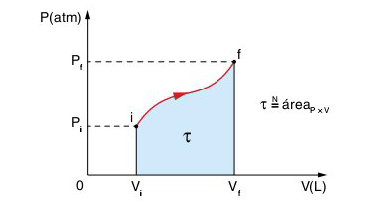
\includegraphics[width=0.7\textwidth]{work.png}
    \caption{A área debaixo do gráfico de Pressão x Volume é numericamente igual ao trabalho feito pelo sistema/gás}
    \end{figure}
    
A energia interna de um gás ideal é dado como:
\begin{equation}
    U= \frac{3}{2}nR T
\end{equation}
\noindent em que 'n' é o número de mols de um gás, 'R' é a constante universal dos gases e 'T' é temperatura (em Kelvin).

A variação da Energia Interna é, então:
\begin{equation}
    \Delta U = \frac{3}{2}nR \Delta T = \frac{3}{2}nR(T_f-T_i)
\end{equation}

\textbf{Essa Primeira Lei da Termodinâmica diz sobre a conservação de energia e de onde vem/vai o calor recebido pelo gás/sistema.}

\item \textbf{2ª Lei da Termodinâmica} - essa Lei fala sobre como o processo de transferência de energia/calor é feito de um corpo para outro. 

\textbf{A primeira parte da Lei é que a troca de calor entre 2 corpos é feita do corpo mais quente para o corpo mais frio, parando somente quando os 2 corpos chegam a uma mesma temperatura (equilíbrio térmico)}.

\textbf{A segunda parte é sobre o rendimento de um processo. Nenhum processo é capaz de transformar todo o calor recebido em trabalho.} O rendimento é dado por:

\begin{equation}
    \eta = \frac{\tau}{Q} = \frac{Q - \Delta U}{Q}
\end{equation}
\noindent em que '$\eta$' (leia-se 'eta') é o rendimento do processo, 'Q' é o calor fornecido, '$\tau$' é o trabalho feito e '$\Delta U$' é a variação da energia interna do gás/sistema.

Por causa da 2ª Lei, $\eta < 1$. O físico francês Carnot, fazendo os seus experimentos, mostrou que o rendimento de qualquer processo respeita a seguinte relação:
\begin{equation}
    \eta_{processo} \leq \eta_{Carnot}
\end{equation}

\noindent em que $\eta_{Carnot}$ é o rendimento de um processo chamado de Ciclo de Carnot, que veremos mais adiante.

\item \textbf{3ª Lei da Termodinâmica} - ela diz que \textbf{é impossível chegar ao 0K com um número finito de processos termodinâmicos (como esfriamento).} \footnote{Na verdade, a mecânica quântica não permite que consigamos chegar ao 0K (zero absoluto), por causa do Princípio da Incerteza de Heisenberg (que diz que não é possível determinar exatamente a posição de uma partícula microscópica. A 0K, as partículas estariam totalmente paradas, sem se movimentar, o que seria possível determinar exatamente a posição das partículas.}
\end{itemize}
\subsection{Transformações especiais - Isotérmicas, Isobáricas e Isocóricas, Adiabáticas}

Vimos na parte de gases que essas transformações elas são especiais pois uma quantidade é mantida constante (a gente verá no fim qual quantidade é constante na transformação adiabática). Veremos como essas transformações são descritas por meio de gráficos de Pressão x Volume.

Para as transformações isobáricas, os gráficos são da seguinte forma:
\begin{figure}[h]
     \centering
     \begin{subfigure}[b]{0.45\textwidth}
         \centering
         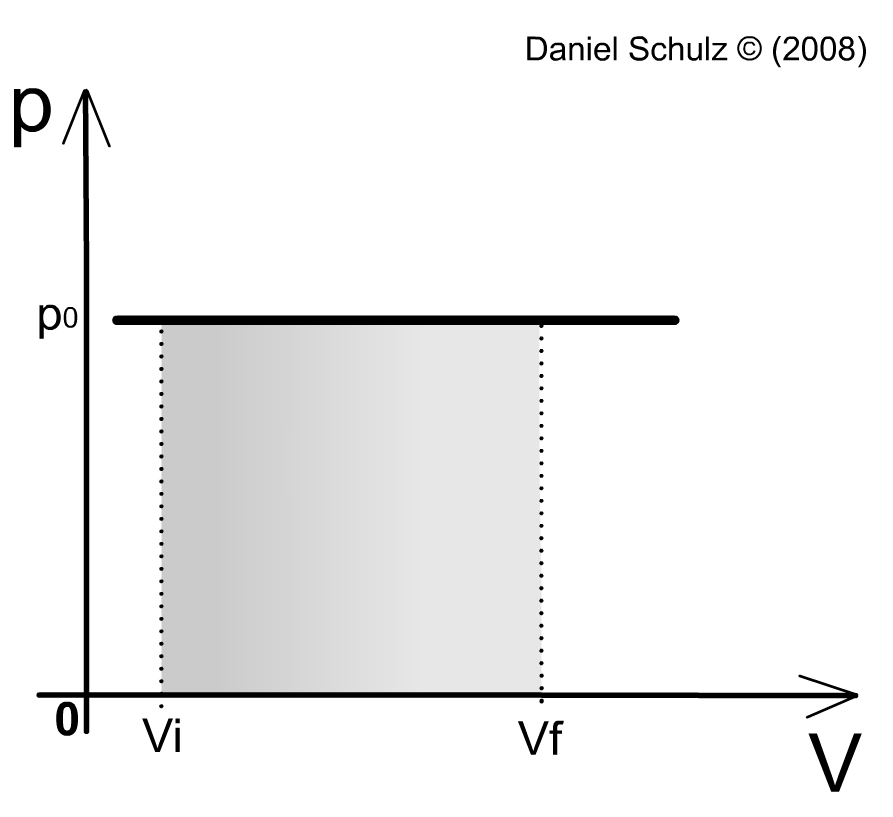
\includegraphics[width=\textwidth]{isobarica_area.jpg}
         \caption{Gráfico da transformação isobárica para o gráfico PxV}
         \label{fig:isobarica_pv}
     \end{subfigure}
     \hfill
     \begin{subfigure}[b]{0.45\textwidth}
         \centering
         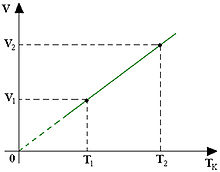
\includegraphics[width=\textwidth]{220px-Diagrama_V_x_T_Transformação_Isobárica.jpg}
         \caption{Gráfico da transformação isobáricas no gráfico VxT. A pressão é determinada como: $P = \frac{V_2-V_1}{T_2-T_1}$}
         \label{fig:isobarica_vt}
     \end{subfigure}
\end{figure}

Para a transformação isocórica/isovolumétrica:
\begin{figure}[H]
     \centering
     \begin{subfigure}[b]{0.45\textwidth}
         \centering
         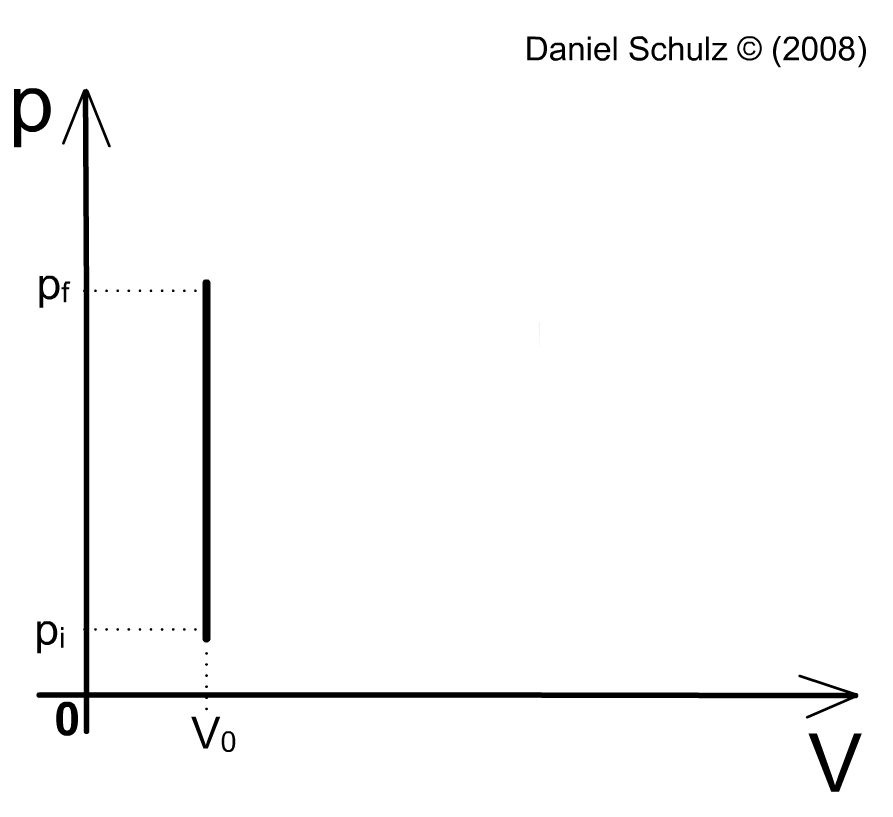
\includegraphics[width=\textwidth]{isocorica.jpg}
         \caption{Gráfico da transformação isocórica num gráfico PxV}
         \label{fig:isocorica_pv}
     \end{subfigure}
     \hfill
     \begin{subfigure}[b]{0.45\textwidth}
         \centering
         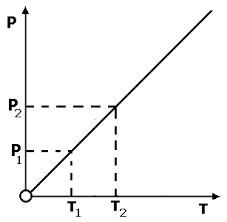
\includegraphics[width=\textwidth]{isovolumetria.png}
         \caption{Gráfico da transformação isocórica num gráfico PxT. O volume é determinado como: $V=\frac{P_2-P_1}{T_2-T_1}$}
         \label{fig:isocorica_pt}
     \end{subfigure}
\end{figure}

Para a transformação isotérmica:
\begin{figure}[H]
     \centering
     \begin{subfigure}[b]{0.45\textwidth}
         \centering
         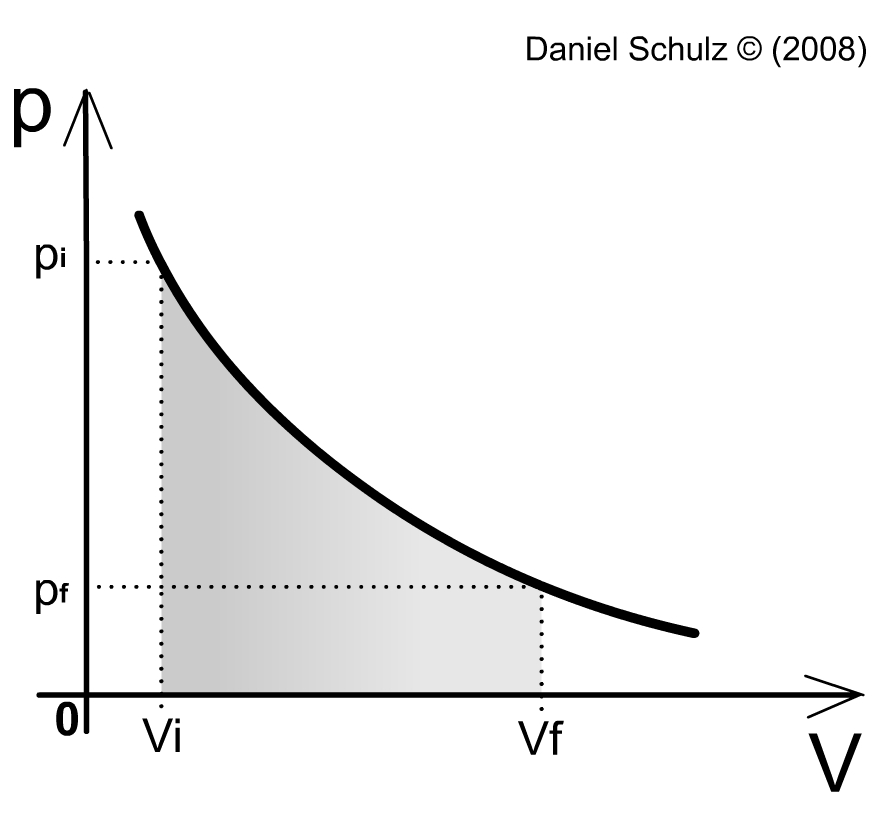
\includegraphics[width=\textwidth]{isoterma_area.jpg}
         \caption{Gráfico de uma transformação isotérmica num gráfico PxV. Sobre a linha, a temperatura é constante.}
         \label{fig:isoterma}
     \end{subfigure}
     \hfill
     \begin{subfigure}[b]{0.45\textwidth}
         \centering
         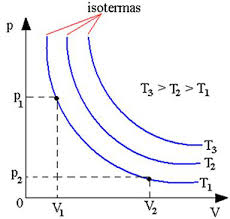
\includegraphics[width=\textwidth]{isotermica.jpg}
         \caption{Vários gráficos de transformações isotérmicas com temperaturas distintas. Quanto maior é a temperatura para cima fica a curva. Importante - elas nunca se cruzam!!!!}
         \label{fig:isotermas_2}
     \end{subfigure}
\end{figure}

Faltou falar sobre as transformações adiabáticas. \textbf{As Transformações Adiabáticas são aquelas que não há calor envolvido, ou seja, Q =0. Importante, isso não implica que a temperatura seja constante, ela varia também!!!!}

Nessa transformação, como Q =0, o trabalho feito é dado por:
\begin{equation}
   0= Q = \tau + \Delta U \implies \tau = -\Delta U
\end{equation}

Numa transformação adiabática, a quantidade constante é a seguinte:
\begin{equation}
    PV^\gamma = constante
\end{equation}
\noindent em que '$\gamma$' (leia-se 'gama') é a constante adiabática e é descrito como:
\begin{equation}
    \gamma = \frac{c_p}{c_v}
\end{equation}
\noindent em que '$c_p$' é o calor específico de um gás à pressão constante e '$c_v$' é o calor específico de um gás à volume constante. \textbf{Caso um enunciado dê o calor específico e não diga qual seja, pode assumir que ele deu o calor específico à volume constante '$c_v$'}

Então, numa transformação adiabática:
\begin{equation}
    P_1\,V_1^\gamma = P_2\,V_2^\gamma \implies \frac{P_1}{P_2} = \left(\frac{V_2}{V_1} \right)^\gamma
\end{equation}

Para gases ideais, $\gamma$ é 5/3. O gráfico dessa transformação é dado por:
\begin{figure}[H]
    \centering
    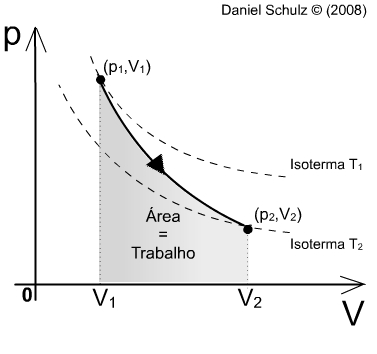
\includegraphics[width=0.4\textwidth]{adiabatica.jpg}
    \caption{Gráfico de uma transformação adiabática num gráfico PxV. Perceba que a curva começa numa temperatura e termina em outra.}
    \label{fig:adiabatica}
\end{figure}

Todas as transformações podem ser resumidas na seguinte imagem:
\begin{figure}[H]
    \centering
    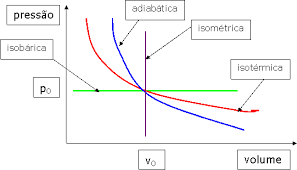
\includegraphics[width=0.7\textwidth]{todas_as_transformacoes.png}
    \caption{Todas as transformações no gráfico PxV}
    \label{fig:pv_transforms}
\end{figure}

\subsection{Ciclos Termodinâmicos}

Podemos fazer uma sequência de transformações de forma que, ao fim delas, voltemos à pressão, volume e temperatura inicial. Quando isso acontece, falamos que a transformação é dita cíclica, pois pode se fazer um ciclo com elas e repetí-las. Fazendo um gráfico de um ciclo:

\begin{figure}[h]
    \centering
    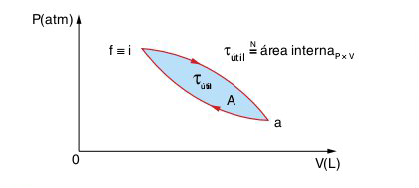
\includegraphics[width=0.6\textwidth]{ciclos_pv.png}
    \caption{Gráfico de um ciclo termodinâmico num gráfico PxV}
    \label{fig:cycle}
\end{figure}

O trabalho feito por um ciclo é a área da figura feita pelo ciclo num gráfico PxV. Na imagem acima, é a área em azul.

\subsubsection{Ciclo de Carnot}
O ciclo mais importante é o ciclo de Carnot, pois ele é o ciclo com maior rendimento (ou seja, faz o máximo de trabalho para uma dada quantidade de calor). Ele foi teorizado por Nicolás Carnot e este ciclo não é possível de ser feito experimentalmente. Este ciclo é um ciclo termodinâmico ideal (quanto mais próximo dele você conseguir fazer, mais eficiente será o seu ciclo).

\textbf{O ciclo é feito de 2 transformações isotérmicas e 2 transformações adiabáticas.}

\begin{figure}[h]
    \centering
    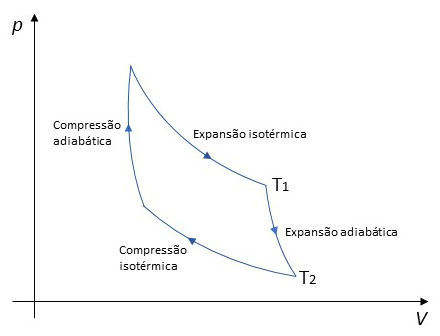
\includegraphics[width=0.6\textwidth]{graficociclocarnot.jpg}
    \caption{Gráfico do Ciclo de Carnot num gráfico PxV. A área dessa figura fechada é o trabalho feito pelo ciclo.}
    \label{fig:carnot}
\end{figure}

O rendimento de um Ciclo de Carnot é dado por:

\begin{equation}
    \eta_{carnot} = 1 -\frac{T_2}{T_1}
\end{equation}
\noindent em que $T_1>T_2$. Quanto mais próximos $T_2$ e $T_1$ forem entre si, pior o rendimento do ciclo. O inverso também acontece e, no limite, $T_1$ muito grande, o rendimento fica muito próximo de 1.
\end{document}
